\chapter{\IfLanguageName{dutch}{Stand van zaken}{State of the art}}%
\label{ch:stand-van-zaken}

% Tip: Begin elk hoofdstuk met een paragraaf inleiding die beschrijft hoe
% dit hoofdstuk past binnen het geheel van de bachelorproef. Geef in het
% bijzonder aan wat de link is met het vorige en volgende hoofdstuk.

% Pas na deze inleidende paragraaf komt de eerste sectiehoofding.

%Dit hoofdstuk bevat je literatuurstudie. De inhoud gaat verder op de inleiding, maar zal het onderwerp van de bachelorproef *diepgaand* uitspitten. De bedoeling is dat de lezer na lezing van dit hoofdstuk helemaal op de hoogte is van de huidige stand van zaken (state-of-the-art) in het onderzoeksdomein. Iemand die niet vertrouwd is met het onderwerp, weet nu voldoende om de rest van het verhaal te kunnen volgen, zonder dat die er nog andere informatie moet over opzoeken \autocite{Pollefliet2011}.

%Je verwijst bij elke bewering die je doet, vakterm die je introduceert, enz.\ naar je bronnen. In \LaTeX{} kan dat met het commando \texttt{$\backslash${textcite\{\}}} of \texttt{$\backslash${autocite\{\}}}. Als argument van het commando geef je de ``sleutel'' van een ``record'' in een bibliografische databank in het Bib\LaTeX{}-formaat (een tekstbestand). Als je expliciet naar de auteur verwijst in de zin (narratieve referentie), gebruik je \texttt{$\backslash${}textcite\{\}}. Soms is de auteursnaam niet expliciet een onderdeel van de zin, dan gebruik je \texttt{$\backslash${}autocite\{\}} (referentie tussen haakjes). Dit gebruik je bv.~bij een citaat, of om in het bijschrift van een overgenomen afbeelding, broncode, tabel, enz. te verwijzen naar de bron. In de volgende paragraaf een voorbeeld van elk.

%\textcite{Knuth1998} schreef een van de standaardwerken over sorteer- en zoekalgoritmen. Experten zijn het erover eens dat cloud computing een interessante opportuniteit vormen, zowel voor gebruikers als voor dienstverleners op vlak van informatietechnologie~\autocite{Creeger2009}.

%Let er ook op: het \texttt{cite}-commando voor de punt, dus binnen de zin. Je verwijst meteen naar een bron in de eerste zin die erop gebaseerd is, dus niet pas op het einde van een paragraaf. \\

Met een digitale elektriciteitsmeter kunnen gezinnen hun elektriciteitsverbruik makkelijk opvolgen. Dat kan in de eerste plaats gratis via het online energieportaal \href{https://login.fluvius.be/klanten.onmicrosoft.com/b2c_1a_customer_signup_signin/oauth2/v2.0/authorize?client_id=91bb9a0a-f45d-491a-ae0b-43324fbc343a&scope=openid%20profile%20offline_access&redirect_uri=https%3A%2F%2Fmijn.fluvius.be%2Fredirect&client-request-id=90c12c72-7d7b-428b-98fc-5d7956e53a60&response_mode=fragment&response_type=code&x-client-SKU=msal.js.browser&x-client-VER=2.23.0&client_info=1&code_challenge=jz-1E8AwB15UEa352eC_5x6zDtAtwp3Je6jrFVdGKjk&code_challenge_method=S256&nonce=cee3d720-d931-4b13-b0b5-c473169ca6fd&state=eyJpZCI6IjRhM2I3M2NkLTgyZjgtNDFjOC05NzAyLTEwMTNjNjNkNjNhMyIsIm1ldGEiOnsiaW50ZXJhY3Rpb25UeXBlIjoicmVkaXJlY3QifX0%3D}{Mijn Fluvius}. Daarnaast bestaan er ook heel wat gratis of betalende online apps die met een digitale meter kunnen verbonden worden om elektriciteitsverbruik op te volgen en eventueel bij te sturen. Zo’n slimme toepassingen heten in het jargon ‘HEMS’ (Home Energy Management System) of ‘CEMS’ (Customer Energy Management System). De aansluiting van deze apps gebeurt via de gebruikerspoorten (P1 en S1) van de digitale elektriciteitsmeter. Beide gebruikerspoorten zijn complementair en geschikt voor verschillende toepassingen. De P1-poort stuurt de elektriciteitsdata per seconde uit. Via de ‘snelle’ S1-poort worden ruwe data aan een zeer hoge frequentie ter beschikking gesteld aan een app of slimme thermostaat. Dit laat gedetailleerde verbruikersfeedback en sturing toe. Recente digitale elektriciteitsmeters hebben evenwel geen S1-poort meer. De verbinding tussen het meettoestel en een app gebeurt in de meeste gevallen via een wifiverbinding of 4G. Een overzicht van deze toepassingen vindt men op de website \href{https://maakjemeterslim.be/}{www.maakjemeterslim.be}.

\section{\IfLanguageName{dutch}{Overzicht functionaliteiten bestaande apps}{Overview functionalities existing apps}}%
\label{sec:overzicht functionaliteiten bestaande apps}

De bestaande apps bieden allemaal de mogelijkheid om elektriciteitsverbruik in real time op te volgen. Zo kan de gebruiker per dag, per week of per maand nagaan hoeveel elektriciteit er verbruikt en/of geproduceerd werd. Het meten van de energiekosten per huishoudtoestel is ook meestal standaard voorzien, maar geldt even vaak als een optie. De meeste apps sporen ook sluipverbruik op en bieden gepersonaliseerde tips voor energiebesparing. Sommige apps bieden tenslotte ook de mogelijkheid om het gemeten elektriciteitsverbruik naast weerdata te leggen en op die manier na te gaan hoeveel stroom men verbruikt bij bepaalde weersomstandigheden \autocite{Deman2021}. Toen ik vorig jaar mijn onderzoeksvoorstel voor deze bachelorproef formuleerde en uitschreef voor het vak 'Research methods' was er nog geen enkele app die de inzichten in het elektriciteitsverbruik gebruikte om automatisch apparten aan te sturen. Het was toen aan de gebruiker zelf om op basis van de gevevens die de app hem toonde actie te ondernemen en toestellen te gaan in- of uitschakelen. Zoals reeds eerder werd vermeld, leidde dit niet altijd tot de gewenste gedragsverandering \autocite{Wemyss2019}, \autocite{Mack2019} en  \autocite{VREG2021}. Ondertussen zijn een aantal apps daarom uitgebreid met de optie om (huishoud)apparaten automatisch in te schakelen via slimme stekkers. Zes apps voorzien momenteel in de optie om toestellen in te schakelen volgens elektriciteitstarieven of het overschot aan zelf geproduceerde stroom van zonnepanelen, daarbij telkens rekening houdend met het piekverbruik zodat een hoger capaciteitstarief vermeden wordt. Dit gebeurt met bijgeleverde slimme stekkers die via wifi kunnen aangestuurd worden. De automatische aansturing gebeurt echter steeds op het moment zelf, wanneer de app merkt dat er een overschot aan elektricteitsproductie is of de elektriciteitsprijzen laag zijn. Tot op heden is er evenwel nog geen app die gebruik maakt van artificiële intelligentie om de zelf geproduceerde zonne-energie te voorspellen. Dit laat de gebruiker immers toe om de vaatwasser of wasmachine op voorhand  in te laden, zodat de automatische aansturing ervan de volgende dag ook effectief kan gebeuren. 

\section{\IfLanguageName{dutch}{Voorspellingen maken met AI}{Making predictions with AI}}%
\label{sec:voorspellingen maken met AI}

Artificiële intelligentie (AI) verwijst naar de mogelijkheid van applicaties of machines om menselijke vaardigheden te tonen, zoals redeneren, leren en plannen. De term AI wordt vaak gebruikt om andere gerelateerde technieken aan te duiden, zoals machine learning (ML) en deep learning. ML en deeplearning kunnen inderdaad onder de verzamelnaam AI vallen, maar omgekeerd is dit niet altijd het geval. De verschillende technieken van AI hebben immers elk hun eigen doel en opzet. Zo is ML bijvoorbeeld gericht op de studie en de ontwikkeling van algoritmen die kunnen leren of hun prestaties kunnen verbeteren op basis van de data waarmee ze gevoed worden. Machine learning is daarom zeer geschikt om voorspellingen te maken op basis van data uit het verleden. 

\subsection{\IfLanguageName{dutch}{Machine learning}{Machine learning}}%
\label{sec:machine learning}

Machine learning kan opnieuw onderverdeeld worden in drie verschillende categorieën, namelijk supervised learning, unsupervised learning en reinforcement learning. 

\subsubsection{Supervised learning}

Bij supervised machine learning wordt een algoritme door de mens aangeleerd welke conclusies het moet trekken. Er wordt daarbij gewerkt met gelabelde data, wat betekent dat voor elke invoer de gewenste uitvoer bekend is. Het doel van het algoritme is om een model te bouwen dat de relatie tussen invoer en uitvoer begrijpt en deze kan toepassen op nieuwe, ongeziene gegevens. Indien een waarde of getal voorspeld wordt, spreekt men van een regressie. Heeft de voorspelling betrekking op een groep of categorie, dan is er sprake van classificatie \autocite{Brownlee2023}. \\

Een voorbeeld van supervised learning is het voorspellen van huizenprijzen. Een model wordt daarbij getraind op een dataset van huizen waarvan de verkoopprijzen bekend zijn, samen met relevante kenmerken zoals locatie, grootte, aantal slaapkamers, enz. Het model leert vervolgens de relatie tussen deze kenmerken en de verkoopprijs van het huis. Als het model dan een nieuw huis met bijhorende kenmerken herkent, zal het de verkoopprijs ervan kunnen voorspellen.

\subsubsection{Unsupervised learning}

Unsupervised machine learning verloopt op een meer zelfstandige manier. Hierbij leert een algoritme om complexe processen en patronen te identificeren zonder de begeleiding van een mens. Bij unsupervised machine learning vindt training plaats op basis van data die geen labels of een specifieke, vooraf gedefinieerde output hebben  \autocite{Brownlee2023}. \\

Het misschien wel meest gekende voorbeeld van unsupervised learning zijn de aanbevelingen die streamingsplatformen zoals Netflix of Spotify aan hun kijkers aanbieden. Algoritmes analyseren het kijk- en luistergedrag van de gebruikers om daarin patronen en voorkeuren te ontdekken. Vervolgens kunnen dan gepersonaliseerde aanbevelingen gedaan worden.

\subsubsection{Reinforcement learning}

Bij reinforcement leert een algortime of cumputersysteem hoe het moet handelen in een omgeving om een bepaald doel te bereiken. Dit gebeurt door het uitvoeren van acties en het ontvangen van feedback in de vorm van beloningen of straffen. Wat reinforcement learning specifiek maakt is dat het leerproces vergelijkbaar is met hoe een mens of dier zou leren door trial-and-error en beloningen \autocite{Efimov2024}. \\

Reinforcement learning wordt gebruikt in robotica, bijvoorbeeld om robots autonoom te laten navigeren in een omgeving. Om een robot obstakels te leren vermijden wordt gewerkt met beloningen en straffen. Voor elke correcte beweging richting het doel zal de robot een beloning ontvangen. Omgekeerd zal de robot bestraft worden voor elke incorrecte beweging die gemaakt wordt. \\

De applicatie die als proof of concept ontwikkeld wordt voor deze bachelorproef, zal de toekomstige stroomproductie van zonnepanelen gaan voorspellen. Hiervoor zullen historische zonnestralingsgegevens gebruikt worden. Er zal dus gebruik gemaakt worden van de supervised learning methode en meer specifiek zal het regressiemodel toegepast worden. De waarde die moet voorspeld worden is de hoeveelheid zonnestraling uitgedrukt in Watt/m².

\subsection{\IfLanguageName{dutch}{Supervised machine learning: regressie modellen}{Supervised machine learning: regression models}}%
\label{sec:supervised machine learning: regressie modellen}

\subsubsection{Decision Tree Regression (DTR)}

Het Decision Tree model is een regressiealgoritme dat een dataset systematisch opdeelt in steeds kleinere homogene subgroepen op basis van de kenmerken van de gebruikte dataset. Het ontwikkelt daarbij een beslissingsboom, waarbij de interne knooppunten de kenmerken van de dataset vertegenwoordigen, de takken de beslissingsregles en elke bladknoop het resultaat. In de beslissingsboom zijn er twee knooppunten, namelijk de beslissingsknooppunten en de bladknooppunten. Beslissingsknooppunten worden gebruikt om een beslissing te nemen en hebben meerdere takken, terwijl Bladknooppunten de uitkomst van die beslissingen zijn en geen verdere takken bevatten.
De beslissingen of de test worden uitgevoerd op basis van de kenmerken van de gegeven dataset. Het doel is om eenvoudige beslissingsregels te leren op basis van die specifieke kenmerken van de dataset om zo een model te ontwikkelen dat een bepaalde waarde voorspelt  \autocite{Balakumar2023}.  
\\
\begin{figure}[h!]
    \centering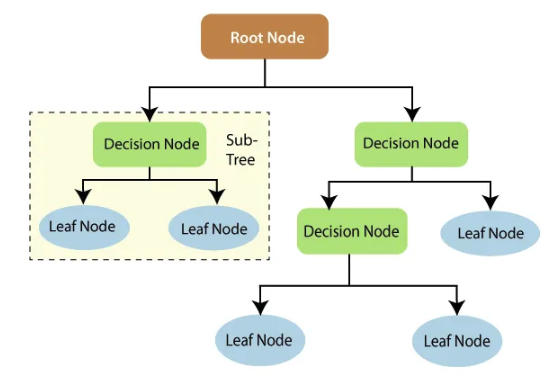
\includegraphics[scale=0.55]{Decision_Tree }
    \caption{\label{fig:Decision_Tree}Grafische voorstelling beslissingsboom.}
\end{figure} 
\\

Decision trees zijn makkelijk te interpreteren omdat de geleerde beslissingsregels makkelijk te begrijpen en visualiseren zijn. Bovendien kan het DTR-algoritme niet-lineaire en dus meer complexe relaties tussen de inputvariabelen en de voorspelde waarde ontdekken, wat het algoritme zeer bruikbaar maakt voor datasets die complexe patronen bevatten  \autocite{Viswa2023}. 

\subsubsection{Random Forest Regression (RFR)}

Het Random Forest regressie model bestaat uit een verzameling van zogenaamde decision trees of beslissingsbomen. Een beslissingsboom is op zijn beurt een schema dat is opgebouwd uit een opeenvolging van binaire beslissingsregels. Het is een grafische voorstelling van een probleemstelling waarin verschillende mogelijke alternatieven met gebeurtenissen worden weergegeven en uitgewerkt. Het RFR-model maakt meerdere beslissingbomen aan op basis van willekeurig gekozen subsets van de gebruikte dataset. Het model voegt vervolgens de uitkomsten van al deze beslissingbomen samen om een algemene voorspelling te doen voor ongekende datapunten. Daarbij wordt telkens het gemiddelde of gewogen gemiddelde van elke beslissingsboom genomen. Op deze manier kan het grotere datasets verwerken en complexere verbanden vastleggen dan individuele beslissingsbomen. Het geheel van de voorspellingen van de beslissingbomen zorgt voor een grotere accuraatheid dan de voorspelling van één enkele beslissingsboom. Over het algemeen kan gesteld worden dat hoe meer beslissingsbomen er in het RFR-model zitten, des te robuster het model zal zijn \autocite{Balakumar2023}. \\

\begin{figure}[h!]
    \centering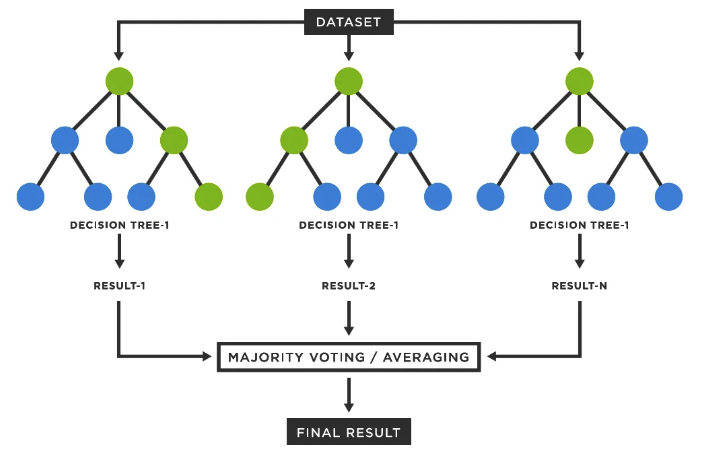
\includegraphics[scale=0.5]{Random_Forest}
    \caption{\label{fig:Random_Forest}Grafische voorstellingvan het Random Forest algoritme.}
\end{figure} 

Het RFR-model wordt vaak gebruikt om continue waarden te voorspellen, zoals aandelenkoersen, tijdreeksen of verkoopprijzen. Het is minder gevoelig voor 'overfitting' (dit doet zich voor wanneer een ML-model de trainingsdata te goed leert, waardoor het nieuwe ongekende data slecht voorspelt) dan andere regressiemethoden omdat het meerdere willekeurige bomen onafhankelijk van elkaar opbouwt en een gemiddelde van de individuele voorspellingen neemt. Het is een goede keuze wanneer data gebruikt wordt met veel verschillende kenmerken of inputvariabelen  \autocite{Sahai2023}.

\subsubsection{Support Vector Machine (SVM)}

Het Support Vector Machine algoritme probeert data zo optimaal mogelijk in twee groepen te verdelen door het vinden van het beste hyperplane. Deze hyperplane is de meest optimale scheidingslijn tussen de twee groepen van data. Het algoritme maakt daarbij gebruik van support vectors. Dit zijn de datapunten die zich het dichtst bij de optimale scheidingslijn bevinden. Om de meest optimale scheidingslijn te achterhalen, berekent het algoritme de maximale marge of afstand tussen de datapunten van de twee groepen  \autocite{Tziolis2024}. Omdat het algoritme zeer effectief is in het oplossen van complexere, niet-lineaire problemen, is het een model dat vaak grbuikt wordt om voorspellingen te maken op het gebied van hernieuwbare energie \autocite{Ahmad2018}. \\

\begin{figure}[h!]
    \centering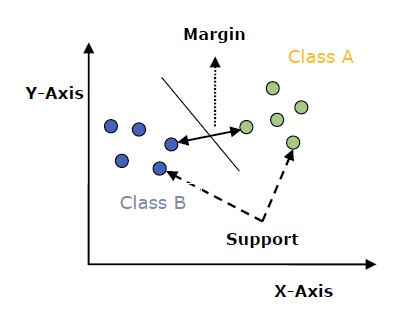
\includegraphics[scale=0.7]{SVM}
    \caption{\label{fig:SVM}Grafische voorstelling Support Vector Machine.}
\end{figure} 

Het SVM-model wordt typisch gebruikt voor kleinere datasets omdat de trainigstijd van dit algoritme zeer lang kan zijn. Het wordt ook vooral toegepast op 'proper' datasets, dit zijn datasets die weinig afwijkingen of fouten bevatten.

\subsubsection{Autoregressive Integrated Moving Average (ARIMA)}

Het Autoregressive Integrated Moving Average (ARIMA) model is een populair voorspellingsmodel voor tijdreeksen. Het wordt veel gebruikt op verschillende gebieden om toekomstige waarden te analyseren en te voorspellen op basis van waarnemingen uit het verleden in een tijdreeksdataset. \\

Het ARIMA-model combineert drie belangrijke componenten: Autoregressie (AR), differentiëren (I) en voortschrijdend gemiddelde (MA). \\

AR - Autoregressief (p): Dit verwijst naar de afhankelijkheid van de huidige waarde in een tijdreeks van eerdere waarden. De volgorde van de AR-component, aangeduid met p, vertegenwoordigt het aantal vertraagde waarnemingen die in het model worden gebruikt. \\

I - Integratievolgorde (d): Dit is het aantal verschillen dat we beschouwen tussen de huidige waarde en de waarde in het verleden om de tijdreeks stationair te maken. Stationair betekent dat de statistische eigenschappen van de reeks, zoals gemiddelde en variantie, constant blijven in de tijd. \\

MA - Bewegend gemiddelde (q): Het vertegenwoordigt de afhankelijkheid tussen de huidige waarde en de restfouten van voorspellingen uit het verleden. Het berekent het gewogen gemiddelde van de vorige voorspellingsfouten. De volgorde van de MA-component, aangeduid met q, geeft het aantal vertraagde voorspellingsfouten weer die in het model worden gebruikt.

\subsubsection{Long Short-Term Memory (LSTM)}

Het Long Short-Term Memory (LSTM) is een type Recurrent Neural Network (RNN) dat wordt gebruikt om temporele afhankelijkheden in gegevens te modelleren. Concreet kan het zich gebeurtenissen uit het verleden of afhankelijkheden uit eerder waargenomen periodes herinneren. \\

Een LSTM is een type netwerk dat speciaal is ontworpen om een computer te helpen informatie langer te onthouden dan gewoonlijk mogelijk is met een terugkerend neuraal netwerk. Het lange-kortetermijngeheugenmodel werkt met behulp van ‘cellen’ die informatie gedurende langere tijd opslaan; wanneer een nieuwe invoer wordt gedetecteerd, worden er nieuwe cellen gemaakt die aan de bestaande cellen worden gekoppeld. Daarnaast kunnen de nieuwe cellen een deel van de informatie die in de bestaande cellen is opgeslagen ‘vergeten’, waardoor het netwerk een deel van wat het heeft geleerd kan ‘vergeten’. \\

\begin{figure}[h!]
    \centering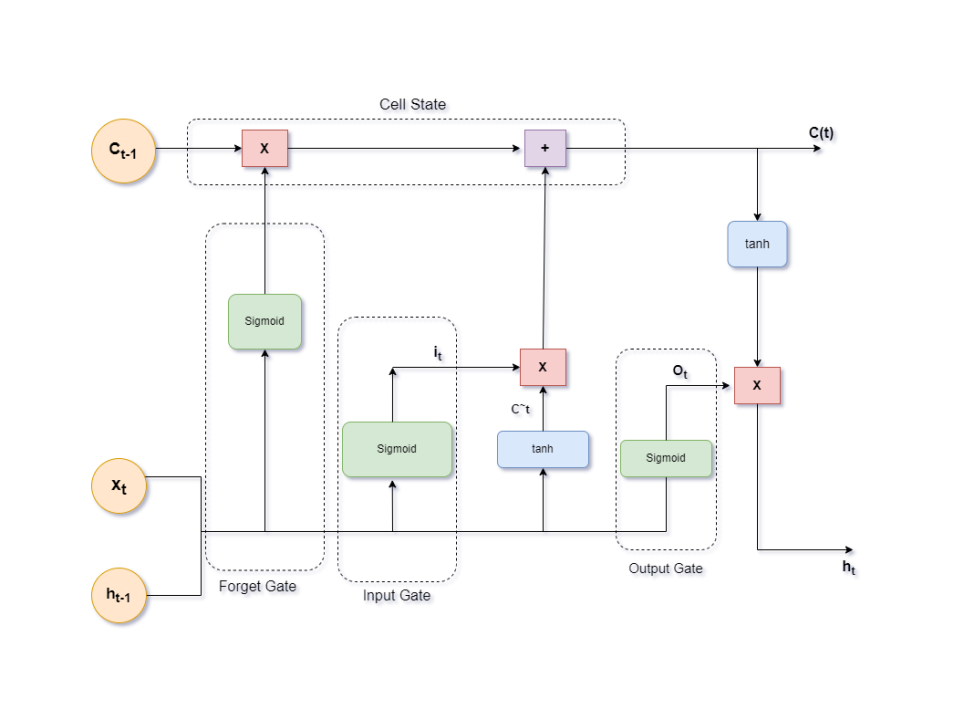
\includegraphics[scale=0.5]{LSTM}
    \caption{\label{fig:LSTM}Grafische voorstellingvan het LSTM algoritme.}
\end{figure} 

De belangrijkste componenten van de LSTM zijn de geheugencellen, vergeetpoorten en invoerpoorten. Geheugencellen zijn verantwoordelijk voor het langdurig opslaan van informatie, en de vergeet- en invoerpoorten beslissen welke informatie wel of niet in de cellen moet worden opgeslagen. Deze componenten zorgen ervoor dat LSTM-netwerken het verleden kunnen ‘herinneren’ en tegelijkertijd rekening kunnen houden met nieuwe input. \\

LSTM's zijn zeer effectief vanwege hun vermogen om informatie gedurende langere tijd op te slaan en nieuwe input efficiënter te verwerken dan traditionele terugkerende neurale netwerken.

\subsubsection{Extreme gradient Boosting (XGBoost)}

Het XGBoost algoritme is een ensemble-leermethode die gradiëntversterking en beslissingsbomen combineert. Het concept van gradiëntversterking verwijst naar het opeenvolgend toevoegen van beslissingsbomen aan het model, waarbij elke volgende boom de fouten corrigeert die door de vorige zijn gemaakt. Dankzij dit iteratieve proces kan het XGBoost zijn voorspellingen voortdurend verbeteren en een hoge nauwkeurigheid bereiken.De werking van beslissingsbomen is hierboven reeds toegelicht. \\

\begin{figure}[h!]
    \centering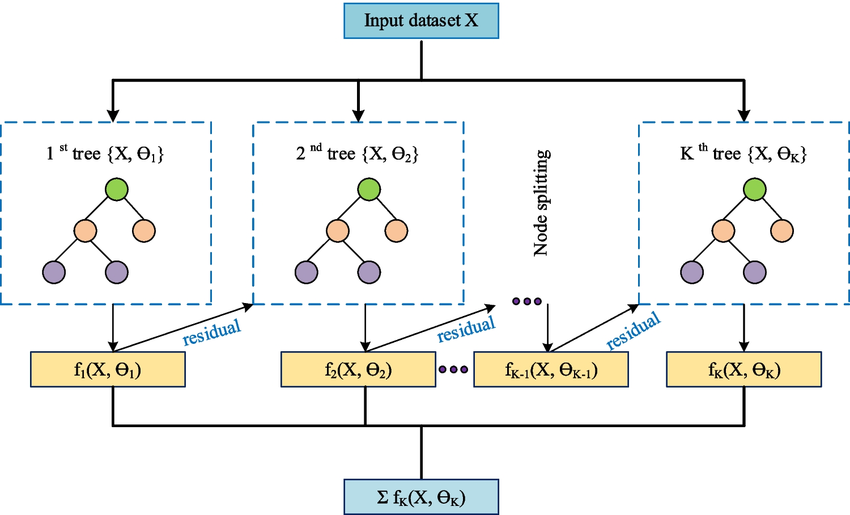
\includegraphics[scale=1.9]{XGBoost}
    \caption{\label{fig:XGBoost}Grafische voorstelling van de structuur van het XGBoost algoritme.}
\end{figure} 

Het XGBoost-model is een open-source implementatie van het gradient boosting algoritme. Het is specifiek ontworpen om de eigen prestaties te optimaliseren en grootschalige datasets efficiënt te verwerken. Door iteratief zwakke voorspellingen toe te voegen, kan het XGBoost algoritme snelle en accurate voorspellingen maken. Het grote voordeel van XGBoost is dat het ingebouwde mechanismen heeft om ontbrekende waarden in de dataset te verwerken. Het kan tijdens het trainingsproces automatisch leren hoe er het beste met ontbrekende waarden kan worden omgegaan. Vermits de meeste datasets uit de echte wereld gegevens ontbreken, is het XGBoost algoritme dus zeer geschikt om voorspellingen te maken. Nog een voordeel van het XGBoost-model is dat het makkelijk schaalbaar is, omdat het gebruik maakt van parallelle verwerkingstechnieken waarbij de werklast over meerdere cores of machines verdeeld wordt. Dit maakt snellere trainings- en voorspellingstijden mogelijk. Deze schaalbaarheid maakt XGBoost geschikt voor toepassingen die realtime voorspellingen vereisen.

\subsection{\IfLanguageName{dutch}{Machine learning modellen evalueren}{Evaluate machine learning models}}%
\label{sec:Machine learning modellen evalueren}

Om een machine learning model te beoordelen wordt de dataset waarmee het model getraid wordt, opgesplitst in een trainingset en een testset. Daarbij wordt de trainigset gebruikt om het model te trainen en wordt de testset gebruikt om de accuraatheid van de voorspellingen van het model te verifiëren. Er bestaan verschillende methodes waarmee de kwaliteit en nauwkeurigheid van een machine learning model kan gemeten worden. De meest gebruikte zijn:

\subsubsection{Mean absolute error (MAE)}

De Mean Absolute Error (MAE) of gemiddelde absolute fout is het gemiddelde van alle absolute voorspellingsfouten waarbij de voorspellingsfout het verschil is tussen de werkelijke en de voorspelde waarde. Het wordt berekend door de absolute verschillen tussen voorspelde waarden en werkelijke waarden bij elkaar op te tellen en te delen door het aantal waarnemingen. Door de absolute waarde van voorspellingsfouten te gebruiken wordt voorkomen dat positieve en negatieve fouten elkaar opheffen. Hoe kleiner de waarde van de MAE, des te beter de voorspellingen van een model overeenstemmen met de werkelijke waarden.

\subsubsection{Mean Squared Error (MSE)}

Mean Squared Error (MSE) of gemiddelde kwadratische fout is de gemiddelde kwadratische afwijking tussen de voorspelde waarden van een model en de werkelijke waarden. Een lagere MSE geeft aan dat de voorspellingen van een model dichter bij de werkelijkheid liggen en het model dus nauwkeuriger is.

\subsubsection{Root mean squared error (RMSE)}

Root Mean Squared Error (RMSE) of vierkantswortel van de gemiddelde kwadratische fout is de gemiddelde omvang van de positieve of negatieve verschillen tussen de waarden die door een model voorspeld zijn en de geobserveerde (feitelijke) waarden. Het kan beschouwd worden als de standaardafwijking van de voorspellingsfouten. \\

RMSE biedt één enkele waarde die de prestaties van een model vertegenwoordigt, waardoor een eenvoudige vergelijking tussen verschillende modellen of voorspellingstechnieken mogelijk is. Lagere RMSE-waarden duiden op betere modelprestaties. Een lagere RMSE geeft aan dat de voorspellingen van het model dichter bij de werkelijke waarden liggen, wat een hogere nauwkeurigheid suggereert.

\subsubsection{R-squared (R²)}

De R-squared (R²) of determinatiecoëfficiënt meet in hoeverre een model in staat is een bepaalde uitkomst te voorspellen. Het geeft aan hoe sterk het verband is tussen de werkelijke waarden en de voorspelde waarden van een model. R² is dan ook nauw verwant aan de correlatiecoëfficiënt. Het kwadraat van de correlatiecoëfficiënt tussen de onafhankelijke en afhankelijke variabelen is gelijk aan de R-kwadraatwaarde. Dit impliceert dat een hogere correlatie overeenkomt met een hogere R-kwadraatwaarde. \\

De laagst mogelijke waarde van R² is 0 en de hoogst mogelijke waarde is 1. Hoe beter een model is in het maken van voorspellingen, hoe dichter de determinatiecoëfficiënt R² bij het getal 1 zal liggen.

\section{\IfLanguageName{dutch}{Elektriciteitsproductie voorspellen}{Predict electricity production}}%
\label{sec:elektriciteitsproductie voorspellen}

Doordat het belang van hernieuwbare energie de laatste jaren enorm is toegenomen, is er al heel wat onderzoek verricht naar het voorspellen van de toekomstige stroomproductie van zonnepanelen met behulp van machine learning. In de meeste van deze onderzoeken wordt deze voorspelling gebaseerd op de voorspelling van de hoeveelheid zonnestraling. \\

Alle onderzoeken opsommen en kort vermelden hoe en wat onderzocht wordt. \\

Een andere optie bestaat erin om de historische stroomproductie van de zonnepanelen te gaan analyseren en daaruit een voorspelling te gaan maken \autocite{Wang2022}. Deze historische stroomproductie data is evenwel niet altijd voldoende voorhanden, zodat het soms niet mogelijk is om op bais daarvan voorspellingen te gaan doen.

\subsection{Zonnestraling}

Vermits zonnepanelen zonne-energie omzetten in elektricteit, is het bijna een logische keuze om de toekomstige stroomproductie van zonnepanelen te gaan voorspellen op basis van de voorspelling van de hoeveelheid zonnestraling \autocite{Ledmaoui2023}. Meestal wordt daarbij de inkomende of globale horizontale instraling (GHI, Global Horizontal Irradiance) voorspeld . GHI is de totale hoeveelheid zonnestraling die het aardoppervlak bereikt en wordt uitgedrukt in W/m². De GHI bestaat uit directe normale instraling (DNI, Direct Normal Irradiance)  en de diffuse horizontale instraling (DHI, Diffuse Horizontal Irradiance). DNI verwijst naar de grootste directe (90 graden) neerwaartse zonnestraling voor een bepaalde plaats. Deze directe normale instraling wordt gebruikt om de diffuse horizontale instraling te berekenen. De DHI is de zonnestraling die niet rechstreeks van de zon komt, maar verspreid is door de wolken en deeltjes in de atmosfeer. Deze zonnestraling komt in gelijke mate uit alle richtingen \autocite{Sehrawat2023}. \\

Historische data met betrekking tot zonnestraling kan vrij verkregen worden via de CAMS Radiation Service (CRS) van de Copernicus Atmosphere Monitoring Service (\href{https://atmosphere.copernicus.eu}{CAMS}). Dit maakt deel uit van het European Earth observation programme Copernicus (EEC) dat informatiediensten biedt op basis van aardobservatiegegevens van satellieten en in-situgegevens (niet uit de ruimte). Enorme hoeveelheden wereldwijde gegevens van satellieten en van meetsystemen op de grond, in de lucht en op zee worden gebruikt om informatie te verstrekken aan dienstverleners, overheidsinstanties, andere internationale organisaties en burgers. De aangeboden informatiediensten zijn gratis en open toegankelijk voor de gebruikers ervan. De geografische dekking van de gegevens is het gebied dat door de Meteosat (een serie geosynchrone weersatellieten van de Europese ruimtevaartorganisaties ESA en EUMETSAT) kan worden waargenomen. Dit gebeid omvat Europa, Afrika en het Midden-Oosten.

\subsection{Meteorologische data}

De hoeveelheid stroom die zonnepanelen produceren is niet enkel afhankelijk van de hoeveelheid zonnestraling. Ook andere meteorologische gegevens spelen hierbij een rol. Zo zijn de temperatuur, de relatieve luchtvochtigheid en de bewolkingsgraad factoren die het meeste invloed hebben op de stroomproductie van zonnepanelen \autocite{Sehrawat2023}. \\

Er zijn verschillende kanalen waarlangs historische weerdata kan verkregen worden. Zo zijn er datasets van meteorologische gegevens die door het Koninklijk Meteorologisch Insituuut (KMI) beschikbaar gesteld worden. Het aantal datasets is echter zeer beperkt en moeten handmatig gedownload worden.Met het oog op de latere integratie van deze data in een app, is dit niet de meest ideale manier. Een andere optie is het CAMS. Ook daar kan historische weerdata voor een specifieke locatie opgevraagd worden, maar deze data is evenzeer beperkt aangezien de meest recente weerdata dateert van 2016. \\

Er bestaan tal van open source en dus gratis weer API's die makkelijk geïntegreerd kunnen worden met een app. Deze API's bieden voorspellingen aan van verschillende meteorologische gegevens, maar leveren vaak beperkte historische weerdata aan. Voor de historische weerdata werd \href{https://dev.meteostat.net/}{Meteostat} gekozen. Deze open-source API biedt een Python library waarmee met slechts een enkele HTTP-request historische weerdata voor een bepaalde locatie kan worden opgevraagd. Meteostat verzamelt historische weer- en klimaatdata van weerstations en verschillende nationale meteorologische instituten van over de hele wereld. De historische weerdata zal voor dezelfde periode als de zonnestralingsdata opgevraagd worden en op die manier de zonnestralingsdata verrijken, zodat de voorspelling van de toekomstige zonnestaling en stroomproductie van de zonnepanelen accurater wordt. \\

De voorspelling van de toekomstige elektriciteitsproductie van de zonnepanelen zal tenslotte nog proberen verbeterd worden door de voorspelde hoeveelheid zonnestraling te combineren met de weersvoorspellingen voor periode die voorspeld wordt. Omdat Meteostat enkel historische weerdata aanbiedt, werd voor de weersvoorspellingen een andere open-source weer-API gebruikt. \href{https://open-meteo.com/}{Open-Meteo API} werkt ook samen met verschillende nationale meteorologische diensten en biedt betrouwbare weersvoorspellingen aan tot 16 dagen in de toekomst. De aangeboden API-request kan makkelijk aangepast worden, zodat enkel de benodigde weerdata kan worden opgevraagd. Dit heeft een gunstig effect op de performantie bij het opvragen van de data.

\section{\IfLanguageName{dutch}{Slimme toestellen aansturen}{Control smart devices}}%
\label{sec:Slimme toestellen aansturen}

Om toestellen automatisch te kunnen inschakelen wanneer er voldoende elektriciteitsproductie van zonnepanelen is, moeten deze toestellen 'slim' zijn. Dit houdt in dat ze over een Soft Real Time Operating System (Soft RTOS) moeten beschikken en via het wifinetwerk kunnen communiceren. Laadpalen voor elektrische voertuigen en warmtepompen, maar ook de nieuwste was- en vaatwasmachines beschikken over deze technologie en kunnen via wifi communiceren. Zij kunnen dus zonder problemen via een app worden aangestuurd. Heel wat bestaande sanitaire toestellen zijn echter niet slim. Daarvoor kunnen slimme stekkers een oplossing bieden. Dit zijn stekkers die via wifi kunnen in- en uitgeschakeld worden. Zij worden tussen het klassieke stopcontact en de stekker van het toestel geplaatst, waardoor een toestel op eenvoudige wijze slim kan gemaakt worden \autocite{Jong2020}. Daarbij stelt zich evenwel het probleem dat een slimme stekker enkel stroom kan doorlaten of tegenhouden. Dit vereist dat een toestel reeds kan ingeschakeld worden indien het geen stroom krijgt en dat het dus zonder tussenkomst van een gebruiker kan opstaren van zodra de slimme stekker stroom doorlaat. Omdat de huidige sanitaire toestellen meestal van stroom moet voorzien zijn om de startknop te activeren, bieden slimme stekkers dus niet altijd een oplossing. \\

\subsubsection{Standaard communicatie protocol}

Een bijkomend probleem dat zich stelt bij de aansturing van slimme toestellen is dat er geen standaard communicatieprotocol bestaat om deze toestellen te laten communiceren met een home energy management system (HEMS). Elke fabrikant gebruikt momenteel zijn eigen communicatieprotocol. Dit maakt dat applicaties die slimme apparaten willen aansturen, een verschillende implementatie per merk moeten voorzien. Het resultaat hiervan is dat een HEMS nodeloos complex kan worden. Daarom wordt binnen Europa gepleit voor een gestandardiseerd communicatieprotocol. De S2 standaard biedt daarbij een oplossing, maar is tot op heden nog niet door Europa goedgekeurd \autocite{Konsman2023a}.